\section{Convergenza globale del metodo di Newton ("delle tangenti") in ipotesi di convessità/concavità stretta}
\underline{Metodo di Newton}: Linearizzare iterativamente la funzione con la tangente nel punto
\[
\begin{cases}
	y = 0 \\
	y = f(x_n) + f'(x_n)(x-x_n) 
\end{cases}
\Rightarrow \,\,\,\,x_{n+1} = x_n - \frac{f(x_n)}{f'(x_n)}
\]
\underline{Convergenza metodo di Newton}:\\
\[
\begin{cases}
	f\in C^2[a,b]\\
	f(a)f(b)<0\\
	f''(x)>0 \,\,\,\,\, \forall x\in [a,b]\\
	x_0 : f(x_0)f''(x_0)>0
\end{cases}
\Rightarrow \underset{\text{e converge all'unico zero $\xi$ di $f$ in $[a,b]$}}{\text{Il metodo di Newton è ben definto (cioè $f'(x_n)\ne 0$)}}
\]
\textbf{Dimostrazione}\\
ci sono 4 casi possibili in base al segno di $f''$ ovvero
\begin{center}
	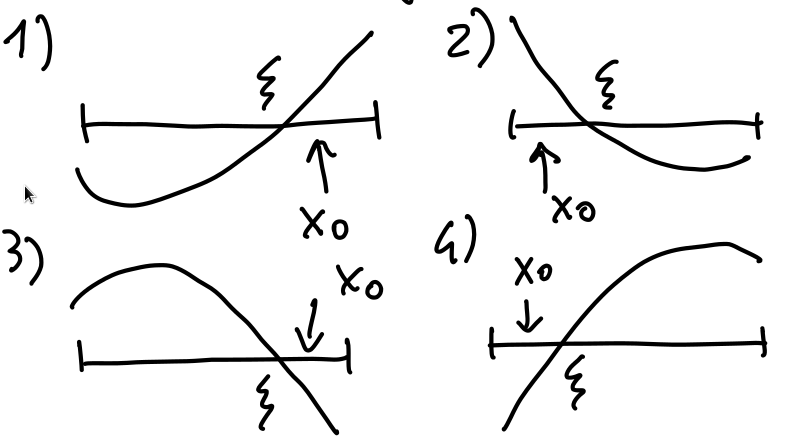
\includegraphics[scale=0.35]{pagina11_1.png}
\end{center}
In questa dimostrazione di concentriamo sul caso 1